%-------------------------------------------------------------------------------------------------------------------------
% Dokument f"ur die ZvL-Geschichte "uber die Wiederentdekcung des San-Titels im SW-Jahre 415.
% Hintergrund ist das die Zauberer von Loh im Jahre 415 ihre eigentlichen Wurzeln nicht mehr pr"asent haben
% und einen Weg suchen ihre alten Traditionen wiedre zu finden.
%
% Autoren: Jan H. Kr"uger, Andre Engelbertz
%
% Erstellt: 20.04.2004
%-------------------------------------------------------------------------------------------------------------------------
% "Anderungen:
% 20.04.2004: Erstellung und grobes Layout
% 21.04.2004: Fortf"uhrung der Geschichte mit Hauptaugenmerk auf die Geschehnisse in der Vergangenheit.
%             "Anderung am Layout, Einf"ugen von FancyHeadern sowie dem ZvL und Olimanir-Logo
% 22.04.2004: Fortf"uhrung, Einbinden der Geschichte um \tiername. Einf"ugen des Glossars.
%
% Geplante "Anderungen: Fortf"uhrung und Abschluss der Geschichte.
%-------------------------------------------------------------------------------------------------------------------------


\documentclass[11pt, twocolumn, a4paper, titlepage]{book}
\usepackage{ngerman, fancyhdr, graphicx}
\setlength{\headheight}{14.0pt}
\pagenumbering{arabic}
\setlength{\parindent}{0pt}
\newcommand{\Charname}{Pummelwurst }
\newcommand{\stadtname}{Woodstock }
\newcommand{\camaronposition}{Camaron }
\newcommand{\Kurzname}{Flitwig }
\newcommand{\samm}{San Achanjati }
\newcommand{\zvl}{Zauberer von Loh }
\newcommand{\tiername}{Vertat }
\newcommand{\andremail}{andre.engelbertz@gmx.de}
\newcommand{\mail}{sir-joker@gmx.de}

\hyphenation {Weges-rand Schauf-fel-zau-ber Phe-ron Zau-ber Ma-gie Mi-no-tau-ren Pum-mel-wurst}

\pagestyle{fancy}

\fancyhead[L]
{ Geschichten der Zauberer von Loh }

\fancyhead[C]
{ }

\fancyhead[R]
{ \LARGE{Der San-Titel} }

\fancyfoot[r]
{ \small{http://www.die-zauberer-von.loh.de/forum} }

\title{ \Huge{Story {\"u}ber die Wiederentdeckung der Sans}}

\author{
    Jan H. Kr{\"u}ger\thanks{\mail}
\and
    Andre Engelbertz\thanks{\andremail}
}
\date{Bad Homburg / K"oppern\\ den \today
%Einf"ugen des Olimanirwappens
\begin{picture}(0,0)
      \put(-60,-310)
      {
         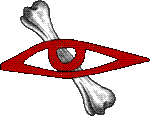
\includegraphics[scale=0.40]{olimanir}
      }
\end{picture}
%Einf"ugen des ZvL-Wappens
\begin{picture}(0,0)
      \put(0,-300)
      {
         
\includegraphics[scale=0.40]{ZvL}
      }
\end{picture}
}

\begin{document}
\maketitle

Die alten M{\"a}nner sa{\ss}en im Kreis zusammen und befragten nun schon zum wiederholten Male die Zukunft. Doch die Bilder welche ihnen ihre gro{\ss}e Kristallkugel zeigen waren auch dieses Mal, wie jedes Mal, von dunklen Wolken {\"u}berzogen. Ein Gewitter w{\"u}rde heraufziehen und dieses Zeitalter beenden. Die Gesichter der Anwesenden wirkten ersch{\"o}pft, selbst das Blau ihrer Roben wirkte blasser. Und ihnen allen war klar: Sie m{\"u}ssten sich auf das kommende vorbereiten.\\

\tiername kroch aus ihrem Bau hervor und reckte sich. Sie Sonne stach anfangs in ihren sich gerade erst wieder an das Licht gew"ohnenden Augen doch langsam erholte sie sich von ihrem Winterschlaf. Der Hunger hatte sie geweckt. Jetzt war sie an die Oberfl"ache gekrochen und hielt ihre keine Schnauze in die Luft. Ihre kurzsichtigen Augen konntes es nicht sehen doch der Schnee war bereits bis auf wenige Stellen welche im Schatten lagen dahingeschmolzen. Dar"uber machte sich \tiername keine Gedanken. Nachdem sie sich gereckt und gestreckt hatte machte sie sich auf die Suche nach N"ussen und anderem Essbaren. Die gro"se Scheibe war bereits freundlich zu ihr, sie froh nicht. Wenn die Scheibe den Sommer hindurch auch so freundlich w"are dachte \tiername, so w"urde dies ein reiches Jahr werden mit vielen fetten Maden und gro"sen N"ussen.\\

\Charname sa{\ss} wie in den letzten Wochen auch in einer herunter gekommenden Taverne am Wegesrand und war {\"u}ber ein B{\"u}ndel Papiere gebeugt. Entt{\"a}uschend waren die Aufzeichnungen, sofern sie {\"u}berhaupt echt waren was \Charname bei manchen doch arg bezweifelte, bisher gewesen. Seit Ende der Unterdr{\"u}ckung und kurz nach der ersten Versammlung der Nachfahren von Loh war \Charname nun schon auf der Reise. Er war sicher seine Augen w{\"u}rden, entweder wenn er seine Aufgabe abgeschlossen hatte oder wenn sein Leben auf dieser Scherbe zu Ende sein w{\"u}rde, was auch immer zuerst kommen m{\"o}ge, wesentlich schlechter sein wie am Anfang. Schon zuviele angebliche Bibliotheken mit angeblich historischen Dokumenten hatte er durchgesehen stets auf der Suche nach ein paar Fetzen von Wahrheit welche Licht in die Vergangenheit der Zauberer bringen k{\"o}nnten. \Charname nahm sich das n{\"a}chste Blatt vor.\\

Eine M{\"o}glichkeit musste gefunden werden wie sie den ersten Ansturm der n{\"a}chsten Jahre {\"u}berstehen mussten. Doch ihre Vorhersagen, ihre ganze Magie, und darin waren sie unbestritten die Meister, verk{\"u}ndete f{\"u}r sie und den Rest der Scherbe nichts gutes. Es waren stets nur nebul{\"o}se Bilder, eine andere, eine starke Macht wirkte primitive M{\"a}chtige Magie welche sich unbemerkt und leise {\"u}ber die gesamte Scherbe ausbreitete. Ihr Ursprung war wild und dennoch waren die Zauberer trotz all ihren Wissens nicht in der Lage die Quelle zu finden. Gestern dann wurden die Tore von T{\'a}n geschlossen und die Stadt magisch verborgen, die Zauberer dieser Stadt begaben sich alle auf die Reise durch die Scherbe um zu lernen. Zu lernen {\"u}ber die Zukunft, zu lernen {\"u}ber die Vergangenheit um sie zusammen mit der Gegenwart zu bewahren auf das die Zukunft beide nicht vernichtete.\\

Die Hinweise in den alten Bl{\"a}ttern hatten ihn also doch nicht in die Irre gef{\"u}hrt. Die Ruinen erstreckten sich {\"u}ber ein weites Feld. \Charname war sicher das eines Tages die Zauberer hier viele interessante Dinge finden m{\"o}gen, Dinge welche nicht durch die Minotauren, die Orks und die Trolle oder danach durch Rattenfra{\ss} vernichtet wurden. Doch heute interessierte ihn nur eine Sache. Er wirkte den Zauber welcher ihn in den letzten Monaten zu eng begleitete. Ja, er hatte ihn richtig gesprochen, er sp{\"u}rte die Anwesenheit von Schriftwerk. Er wanderte durch die Ruinen bis er meinte die richtige Stelle gefunden zu haben. Das folgene w{\"u}rde er ohne seine Magie schaffen m{\"u}ssen. \Charname nahm die Schauffel zur Hand. M{\"o}ge Pheron den Zauberern inspiration schenken und sie einen Zauber zur Belebung von Schaufeln entwickeln lassen. Hoffentlich waren es nur nicht wieder alte Lob- oder Schm{\"a}hreden {\"u}ber den reichen K{\"o}nig, manchmal wurde er auch Dieb genannt, Kokosnuss.\\

Ein Jahr war nun vergangen und es war keine L{\"o}sung gefunden worden. Keine welche die Zauberer und ihr Wissen bewahren mochte. Pheron stellte sie vor ihre gr{\"o}{\ss}te Pr{\"u}fung denn bisher brachten alle ausgesandten Zauberer nur Niederlagen und Entt{\"a}uschungen zur{\"u}ck. Selbst die gr{\"o}{\ss}te Hoffnung der Zauberer, diese Scherbe zu verlassen und in einer anderen Zuflucht zu suchen schlossen sie aus. Es stand zu bef{\"u}rchten das die Urheber der unbekannten Macht die Ver{\"a}nderungen im Managef{\"u}ge beim Verschwinden der Zauberer bemerken w{\"u}rde und ihnen dann auf die andere Scherbe folgen w{\"u}rde. Sie konnten es nicht verantworten eine weitere Scherbe dieser unbekannten Gefahr auszusetzen. Es begann zu regnen und der alte Zauberer, durch die langen Studien bereits gebeugt, ging wieder in sein Studierzimmer. Weitere M{\"o}glichkeiten mussten gepr{\"u}ft werden.\\

\Charname betete zu Pheron er m{\"o}ge nicht noch weiter graben m"ussen.
\Charname betete zu Pheron er m"oge die Inspiration der Zauberer st{\"a}rken und ihren Fokus auf den von ihm gew{\"u}nschten Schauffelzauber richten.
Diese Schriften waren tief verborgen. Wer auch immer diesen Turm baute, er war fr{\"u}her einmal mit vielen Stockwerken ausgestattet. Und mit einem weitreichendem Keller. Pheron, bitte steh deinen treuen Dienern bei.\\

Ohja, die Scheibe war dieses Jahr freundlich gewesen. \tiername hatte viele und vor allem fette Maden in dem Baum welcher letztes Jahr bei einem Sturm entwurzelt wurde gefunden. Heute lag sie vor ihrem Bau und hatte alle sechse von sich gestreckt w"ahrend sie eine Biene beobachtete die um eine gelbe Blume tanzte. Eigentlich waren sie gar nicht so verschieden dachte \tiername. Auch die Biene sammelte den Sommer "uber Vorr"ate und baute ihren Bau aus wie sie es getan hatte. Eine sch"one neue H"ohle hatte sie gebuddelt und mit reichlich Moos und Gras ausgelegt. Ja, das w"urde ihrem Nachwuchs gefallen. Weiter tr"aumend lauschte \tiername dem Summen der Biene.\\

\samm stand an der K{\"u}ste von Almaren und blickte auf das bewegte Meer hinaus. Und weiter. Olimanir sprach wieder zu ihm, doch was sie sagte gefiel weder ihm noch ihr. Gewitter zog herauf doch \samm wusste das sie kein gew{\"o}hnliches Gewitter meinte. Es w{\"u}rde wild werden und die ersten Tropfen versprachen ihr neue, kr{\"a}ftige K{\"o}rper doch der Donner w{\"u}rde auch ihre Diener hinwegfegen. Etwas wildes breitete sich aus dem Westen aus und drang nach Osten auf die gro{\ss}en Metropolen zu. Etwas was auch Olimanir nicht genau benennen konnte. Achanjatis leere Augenh{\"o}hlen senkten sich zu Boden. Was sie ihm sagte gefiel ihm nicht und er bekam Angst um seine Freunde.\\

Er z{\"u}ndete sich eine neue Pfeife an. Pheron hatte sich in diesen Tagen etwas gn{\"a}dig gezeigt. Durch Verhandlungsgeschick war es ihnen m{\"o}glich ein B{\"u}ndniss mit Walnut aus zu handeln, Bearpaw und die Zauberer von Loh w{\"u}rden von nun an zusammen arbeiten. Dies gab ihnen die dringend ben{\"o}tigte Zeit sich auf das Problem zu konzentrieren w{\"a}hrend ihnen das B{\"u}ndniss mit Bearpaw den R{\"u}cken ein wenig frei hielt. {\"A}hnliche B{\"u}ndnisse und Abmachungen wurden bereits vorbereitet um den Zauberern den Weg frei f{\"u}r ihre Studien zu machen. Er lehnte sich in seinem Sessel zur{\"u}ck. Aber jetzt w{\"u}rde er ein wenig schlafen. Schlaf war ein Luxus den er sich in den letzten Wochen nur sp{\"a}rlich g{\"o}nnte. Selten war er so schnell eingeschlafen.\\

Oh Pheron, womit habe ich das nur verdient. \Charname hatte sich nun schon bis an sein Ziel durchgearbeitet. Er war in einer noch halbwegs gut erhaltenen B{\"u}cherkammer angelangt doch seine erste Entdeckung war eine dicke Ratte gewesen welche es sich inmitten eines gro{\ss}en Buches bequem gemacht hatte und ihn ob seiner St{\"o}rung frech anfauchte. Der schnell gewirkte Eiszauber l{\"o}ste zwars das Rattenproblem doch \Charname glaube nun fest das diese Ratte mit System gehaust hatte. Das Buch an dem sie sich verging war die Inventarliste gewesen. Nun musste er selbst alle noch erhaltenen B{\"u}cher durchforsten. Er wusste es. Er hatte es gewusst. Sein schlimmster Feind hatte wieder zugeschlagen. Rattenfra{\ss}.\\

M"ude und gl"ucklich blickte \tiername auf ihren Nachwuchs. 9 kr"aftige und gesunde B"alger welche nun friedlich in der Kinderh"ohle schliefen. \tiername war froh das die Sonne so freundlich war und ihr erm"oglichte einen gro"sen Vorrat anzulegen. So musste sie jetzt nicht mehr hinaus.\\

[Zwischensequenzen einf{\"u}gen]\\

\Charname hatte es geschafft. Nach monatelangem Suchen und W{\"a}lzen von staubigen Schriften hatte er erstmals eine tats{\"a}chliche Spur. Die B{\"u}cher dieser B{\"u}cherkammer sprachen davon das die alten Zauberer das End ihrer Zeit sahen. Eine dunkle Macht breitete sich damals auf der Scherbe aus. \Charname war nun sicher das die \zvl die Unterdr{\"u}ckung voraus sahen und etwas unternahmen um nicht der Vernichtung anheim zu fallen. Best{\"a}rkt hierdurch verga{\ss} er die ganze bisherige plakerei und versp{\"u}rte neue Kr{\"a}fte durch seinen K{\"o}rper fliessen. Erst einmal musste dieser Raum gesichert werden. Schliesslich wollte \Charname ja nicht riskieren morgen fr{\"u}h eine Ratte noch ein weiteres Buch zerst{\"o}ren zu sehen. So machte er sich auf die Suche und gegen Abend schaffte er es dann auch da Schlupfloch welches die Ratte genutzt hatte um einzudringen zu finden und zu versiegeln. Danke Pheron, wenigstens diesesmal gabest du uns einen praktischen Zauber. F{\"u}r heute war es jedoch genug und \Charname nahm sich vor morgen, frisch ausgeruht die B{\"u}cher nach weiteren Hinweisen zu durchforsten.\\

[Zwischensequenzen einf{\"u}gen]\\

Der Rat der Zauberer stimmte zu. Sie durften nicht leichtfertig ihr Verm{\"a}chtnis demjenigen in die Hand legen welche das Artefakt zuerst fand. Es m{\"u}ssten also Sicherheitsvorkehrungen getroffen werden welche verhindern das der Rat von unbefugten aus seinem Schlaf geweckt wurden. Es d{\"u}rfte nur jemand sein in dem die Magie auch fliesst. Weiterhin sollte sichergestellt werden das nur Nachfahren der Zauberer oder jemand von ihrem Geiste den Rat wecken d{\"u}fen.\\
Es galt also sich Gedanken um die Sicherheit zu machen. Weiterhin war die letztendliche Art des Artefaktes noch nicht sicher. Das Ritual musste vorbereitet werden. Der Weg welcher von \samm genutzt wurde kam nicht in Frage. Die Zauberer wollte so lange wie m{\"o}glich Widerstand leisten und das erforderte das ihr Transferritual m{\"o}glichst schnell gewirkt werben konnte. Weiterhin musste ein sicherer Aufbewahrungsort gefunden werden. Sie durften nicht riskieren das die Urheber, wer auch immer es sei, das Artefakt fanden. Ja, viel musste noch getan werden und ihnen blieb immer weniger Zeit.\\

[Zwischensequenzen einf{\"u}gen]\\

Nach langen {\"U}berlegungen hatten sie sich endlich geeinigt. Wie schon im Quellritual hat der Rat beschlossen eine Kugel zu nehmen. Doch das Ursprungsritual musste vollkommen umstruckturiert werden. \samm`s Seelenkugel war nur darauf ausgelegt eine Seele in eine Kugel zu bannen. Doch was die Zauberer vor hatten war gr{\"o}{\ss}er. Gewaltiger. Manche Ratsstimmen sprachen schon von den Grenzen des Wahnsinns. Doch eine Alternative hatten auch sie nicht. Das Ritual warf immer noch gro{\ss}e Probleme auf. Zum Beispiel musste gew{\"a}hrleistet sein das die Seelen w{\"a}hrend des Transferes nicht zu einer gro{\ss}en Seele verschmolzen werden. Andererseits wollten alle Beteiligten das die Seelen untereinander ebenfalls kommunizieren k{\"o}nnten und dennoch wollten sie sicherstellen das jeder sich auch zur{\"u}ckziehen kann. Eine schwierige Aufgabe.\\

[Zwischensequenzen einf{\"u}gen]\\

Die Urheber des heraufziehenden {\"U}bels wurden nun endlich gefunden. Wie die Zauberer in Erfahrung bringen konnten bereiten die Schamanen ein fremdes Ritual vor, sie konzentrieren ihre M{\"a}chte. Gleichzeitig sind zahlreiche Minotauren bei Stonebear Caldera gelandet und haben mehrere Br{\"u}ckenk{\"o}pfe errichtet. Die ersten Versuche sie zur{\"u}ck zu schlagen schlugen fehl. Offensichtlich sch{\"u}tzt m{\"a}chtige Magie die Lager. Weder rohe Gewalt noch ausgekl{\"u}gelte Analyse des die Lager umgebenden Manaflusses erbrachte Hoffnung gebende Resultate. Trotz allem kannten sie nun ihren Feind. Das die Schamanen der Minotauren {\"u}ber gro{\ss}e Magie verf{\"u}gten dar{\"u}ber wurde bereits kurz nach ihren ersten Sichtungen {\"o}ffentlich von den Gelehrten Abakus und \samm diskutiert. Wie sonst h{\"a}tte ihre Insel so pl{\"o}tzlich mitten im Meer auftauchen k{\"o}nnen? Fraglich bleibt nur ob sie schon immer dort waren oder die F{\"a}higkeit ihre Insel zu bewegen besitzen. Beides l{\"a}sst allerdings auf m{\"a}chtige Magie schliessen. Und es bedeutet das die Minotauren intelligenter sind als bisher angenommen.\\

[Zwischensequenzen einf"ugen]\\

Die Truppen waren bereits sehr nahe ger"uckt. F"ur \camaronposition war es nun h"ochste Zeit, die anderen waren bereits gegangen und waren in der Seelenkugel aufgegangen. Sie hatten bis zum letztm"oglichen Zeitpunkt ausgeharrt und der Scherbe all die Hilfe gegeben die sie ihr geben konnten. Es war ihnen sogar gelungen mehrere der zeitgleich mit der gro"sen Offensive auftretenden D"amonen aus den niederen Scherben zu bezwingen. Und dennoch hatte das Land schwer gelitten soweit sie es bisher sehen konnten. Es blutete f"ormlich, es war verbrannt und die Erde tat sich auf und gl"uhende Lava ergo"s sich "uber das Land wo auch immer die D"amonen hinkamen. M"oge dies reichen um die Scherbe vor der Vernichtung zu bewahren. Sie hat gelitten und wird noch st"arker leiden doch so Pheron will m"oge sie weiter bestehen. Er h"orte bereits die Horden der Orks an die "au"seren Tore schmettern. Sie waren nicht sehr effizient vorgegangen doch das hatten sie mittels Gewalt und purer Ma"se mehr als wett gemacht. Ja, es wurde Zeit. \camaronposition begab sich zur Seelenkugel und sprach die Worte welche die Kuppel des Saales "offnete und den Blick auf den freien Himmel freigab. Nun w"urde er seine letzten beiden Zauber f"ur eine sehr lange Zeit sprechen. Vielleicht f"ur immer. Er l"oste den ersten, noch unter Anwesenheit der anderen Zauberer gewirkten Zauber aus welche die Vernichtung bringen w"urde. Er lauschte in die Stille. Dann h"orte er den Beginn dessen was sich innerhalb der n"achsten Bur von den "au"seren Grenzen der lohischen Grenzen bis ins Zentrum, bis hierher fortsetzen w"urde. Eine m"achtige Manawalze w"urde unaufhaltsam hierherrollen und alles einebnen was sich ihr in den Weg stellte. Alles w"urde vernichtet, nichts w"urde mehr da sein was den Minotauren n"utzen k"onnte. Es schmerzt \camaronposition die sch"onen Bauten der Zauberer, ihre gro"sen Labore und Bibliotheken vernichtet zu sehen. Doch es musste sein. Nichts dergleichen durfte den Minotauren in die H"ande fallen.\\Er wirkte den zweiten Zauber. Es geschah anders als er sich vorgestellt hatte. Ein Zerren und ziehen breitete sich in seinem ganzen K"orper aus. Dann folgte eine gro"se Erleichterung. Die schweren Lasten der letzten Monate fielen von seinen Schultern ab und ein tiefern Seufzer entfuhr seinem sterbendem Leib. Dann sp"urte er nichts mehr. Eine Leere brach auf ihn herein, "ahnlich wie es von \samm angenommen wurde. Eine kurze Desorientierung. Dann f"uhlte er sie. Sie kamen um ihn willkommen zu hei"sen. Alle Zauberer welche sich f"ur diesen Weg entschieden hie"sen ihn in ihrem neuen Leben willkommen. \camaronposition fing sich wieder. Er f"uhlte neue Kr"afte durch ihn flie"sen. Nein, durch seinen Verstand. Befreit von den H"urden der Sterblichkeit und eines K"orpers begann sein Geist sich voll auszubreiten. Es w"urde interessant werden.\\

In der Zwischenzeit wurde der zweite Teil des ersten Zaubers ausgel"ost. Er schleuderte die Kugel hoch in die Luft und w"urde sie weit fortschleudern. Der Segen und die Hoffnung aller Zauberer lag in ihr auf das ihre letzten beiden Verb"undeten, Pheron und die Magie, den Flug der Kugel lenken w"urden damit sie eines Tages von den bestimmten Empf"angern gefunden wurde. Die heranst"urmenden Horden der Orks erstarrten kurz in ihrem Sturm auf diese m"achtige Feste vor der die Schamanen der Minotauren sie gewarnt hatten. Ein heller Stern erhob sich aus dem zentralen Geb"aude und stieg immer h"oher bis er dann gen Norden sauste bis er nicht mehr zu sehen war. Dann setzten sie ihr Zerst"orungswerk fort.\\

\Charname hatte alles zum widerholten Male "uberpr"uft. Dies war seine vielversprechendste Stelle und er war sicher das Pheron ihn nicht entt"auschen w"urde. Andere Zauberer waren an weniger vielversprechende Orte geschickt um zu suchen doch \Charname dachte das dies alles nicht erfolgreich war. Anders hier. Hier, das sp"urte er f"ormlich, w"urde er diesesmal f"undig. Weit war er nun schon gereist und hatte sich durch unbewohnte Gegenden geschlagen, hatte gelernt auf welche Dinge er achten musste wenn er verborgene Sch"atze suchte. Seit Burs suchte er bereits hier, von oben bis unten sah er mittlerweile mehr wie ein W"uhlschrat denn wie ein Zauberer aus. Seine Zauber verrieten ihm das hier ein m"achtiges Artefakt verborgen war. Doch sonstiges war im nicht bekannt. \Charname hoffte nur das es nicht wieder eine Putzwolke sei wie das Artefakt welches er in den n"ordlichen Eisgletschers fand, eingefroren und ein wenig angegraut. Ein seltsamer Magier musste sie geschaffen haben. Sie nahm das reinigen so ernst das sie ihn Anfangs schockierte als sie sogar versuchte die Tinte seiner Aufzeichnungen wieder zu entfernen. Aber diesesmal sp"urte er das er richtig lag. Es musste einfach so sein. Pl"otzlich stiess seine Schauffel auf Widerstand. Seltsam, in dieser Gegend gab es doch gar keine Steinvorkommen. Er legte die Schauffel beiseite und untersuchte den Gegenstand. Er war stark verkrustet und unter Ablagerungen verborgen aber dennoch war klar zu erkennen das er eigentlich rund war. Zu rund. \Charname buddelte mit den H"anden weiter. Eine Bur sp"ater reiste er mit schwerem Gep"ack auf dem schnellsten Weg zu den anderen Zauberern.\\

In \stadtname angekommen sprach \Charname sofort mit \camaronposition "uber seinen Fund. Beide stimmten zu das dieser Fund von gr"o"ster Wichtigkeit sei und umgehend alle Zauberer benachrichtigt werden m"ussen. W"ahrend \Charname sich auf Gehei"s von \camaronposition daran machte den Fund f"ur die anstehenden Untersuchungen durch die Versammelten Analysten der Zauberer vorzubereiten begab sich \camaronposition in den mystischen Zustand des Lupu. Jener Zustand welcher es Angeh"origen der f"ahigen Zaubererkaste erm"oglicht ihren Geist von ihrem K"orper zu l"osen um so andere Orte aufzusuchen oder in dieser besonderen Ebene mit den anderen Zauberern in Kontakt zu treten. Zwei Stunden sp"ater begaben sich die meisten Zauberer auf den Weg gen \stadtname.

\begin{quote}
[Was folgt...]
Hier sollte nun noch kommen die ZvL haben das Artefakt gereinigt und untersucht, es ist die Seelenkugel welche in den Aufzeichnungen von \Charname gefunden wurde (entsprechenden Text an eine der Stellen bei Zwischensequenzen einf"ugen) welche nun in einem Labor der ZvL kr"aftigst untersucht wird doch es ist den Zauberern keine Aktivierungsm"oglichkeit eingefallen. Mir auch nicht. Jemand Ideen? Nach Aktivierung meldet sich der Rat zu Wort. macht viel Blabla, "Offner muss ein geistiger Nachfahre der alten Zauberer sein, erz"ahlt was sie gemacht haben um ihr Wissen f"ur die Nachwelt zu erhalten und das fortan der Rat der Zauberer von L"oh sie begleiten m"oge und ernennen einen der Anwesenden zum San warum auch immer m"usst ihr "uberlegen und dann noch der Abspann die ZvL treten alle in blauen Gew"andern an die "Offentlichkeit und Verk"unden einen Text das sie Wiederaufgestanden sind und blablablub.\\
Alternativ ist es auch m"oglich das nicht \camaronposition die letzten Zauber spricht sondern \samm. Er wird nicht in der Seelenkugel aufgehen sondern in Olimanirs Reich eingehen. Das ist bereits zu vollzogen. Die Herrin der Seelen kann man nicht die verlangten Seelen vorenthalten ;)
Nebenbei sollte "uberhaupt "uberlegt werden ob alle ZvL dort eingehen oder es Ausnahmen gibt.
\end{quote}

\onecolumn
\begin{center}
\LARGE{Glossar}
\end{center}

%Glossar mit wichtigen Begriffen
\begin{description}
\item[Clepsydra]Vergleichbar mit einer Sanduhr, einziges Zeitmessger�t.
\item[Dom]Freundschaftliche Anrede. Gleichzusetzen mit Kumpel.
\item[Dopa]Ein feuriger Schnaps, der einen in k"ampferische Extase treibt.
\item[Eisgletscher von Sicce]Dorthin kommt die Seele wenn man stirbt.
\item[Jikai]Bezeichnung f"ur einen schwierigen Kampf.
\item[Jikaida]bevorzugtes,sehr beliebtes Brettspiel.
\item[Kapt]Bezeichnung f"ur einen Armeegeneral.
\item[Ib]Geist und Seele.
\item[Lahal]Offizielle Begr"u"sungsanrede unter den Zauberern von Loh. F"ur Freunde gedacht im Unterschied zu Llahal.
\item[Leem]Verabscheuungsw"urdige Gottheit der Kinderopfer gebracht werden.
\item[Llahal]Formelle Begr"u"sungsandre f"ur Fremde.
\item[Llanitsch]Halt!
\item[Loh]Tropfenf"ormiger Heimatkontinent der Zauberer von Loh.
\item[Lupu]Zustand in den ein Zauberer sich versetzt um an einem anderen Ort etwas auszuspionieren oder jemandem etwas mitzuteilen.
\item[Luz]Grosse rote Sonne.
\item[Lynxter]Lohisches Schwert.
\item[Paktun]Anderes Wort f"ur S"oldner.
\item[Remberee]Abschiedsfloskel welche von den Bewohnern von Loh benutzt wird. Vergleichbar mit Auf Wiedersehen.
\item[San]Titel der f"ur Weiser/Gelehrter steht und Zauberern/Priestern verliehen wird.
\item[Sazz]Alkoholfreies Getr"ank das gut den Durst l"oscht.
\item[Walfarg]Grosses Reich von dem einst Loh den Mittelpunkt bildete.
\item[Walig]kleine gr"une Sonne.
\item[ZvL]Abk"urzung f"ur Zauberer von Loh.
\end{description}

\end{document}

